\documentclass[a4paper, 14pt]{extarticle}
\usepackage[left=2cm,right=2cm,top=2cm,bottom=2cm,bindingoffset=0cm]{geometry}
\usepackage[utf8]{inputenc}
\usepackage[english, russian]{babel}
\usepackage{amssymb, latexsym, amsmath}
\usepackage{indentfirst}
\usepackage{graphicx}
\usepackage{citehack}
\usepackage{tabularx}
\usepackage{listings}
\usepackage{pdfpages}

\lstloadlanguages{HTML,python}
\lstset{extendedchars=false,
  breaklines=true,
  breakatwhitespace=true,
  keepspaces = true,
  tabsize=2
}


\begin{document}
\begin{titlepage}

\newpage

\begin{center}
Московский Авиационный Институт \\*
(национальный исследовательский университет) \\*

\vspace{2em}

Факультет прикладной математики и физики \\*
Кафедра вычислительной математики и программирования

\vspace{10em}

\Large \textbf{Курсовой проект \\*
по дисциплине <<Информационные технологии в проектировании и производстве>>} \\*

\vspace{3em}

<<Разработка проектного офиса <<Цифромед>>
\end{center}

\vspace{8em}

\hspace{25em}\vbox{
  \hbox{\bfseries{Выполнил:}}
  \hbox{\hspace{1em} Данилычев И.\,А.}
}

\vspace{2em}

\hspace{25em}\vbox{
  \hbox{\bfseries{Руководитель:}}
  \hbox{\hspace{1em} Скородумов С.\,В.}
}

\vspace{\fill}

\begin{center}
Москва, 2015
\end{center}

\end{titlepage}

\newpage


\tableofcontents
\newpage


\section{Аннотация}
При компании <<Скородумов и Партнеры>> был сформирован отдел проектирования программного обеспечения, специализирующийся на создании интернет-решений для малого и среднего бизнеса, образовательных учреждений, госпредприятий, задачей которого стала разработка офиса управления проектами, позиционирующегося как SaaS-приложение (Software as a Service, или <<ПО как услуга>>).

Результатом работы над проектом стало появление на свет проектного офиса <<Цифромед>>, представленного в виде веб-приложения, реализованного на языке Python с применением многофункционального фреймворка Flask.

Одной из целей проекта также являлось обеспечение компании <<Скородумов и Партнеры>> решением для управления проектами, предназначенным для внутреннего пользования и при этом, несмотря на имеющиеся аналоги (teamtools.ru, <<Мегаплан>> и др.), не уступающим им по основным показателям производительности и функциональности.


В данный отчёт входят:

\begin{itemize}
\setlength{\itemsep}{-1mm}
\item Иерархическая модель работ (WBS, Work Breakdown Structure) и бизнес-модель проекта;
\item IDEF0-модель цикла разработки данного проекта;
\item Техническое задание;
\item Структура базы данных приложения;
\item Программная логика серверной части (backend);
\item Описание интерфейсной части (frontend);
\item Паспорт проекта и его данные.
\end{itemize}

\newpage


\section{Анализ проекта}
\subsection{Цель проекта}

Ни для кого не секрет, что грамотное планирование в совокупности с тайм-менеджментом и распределением ответственности, зачастую реализуемым через методологию иерархической структуры проекта (Work Breakdown Structure), являются <<сердцем>> любого проекта и в основном определяют успешность его жизненного цикла вкупе с полнотой.

Целью данного проекта являлось создание веб-сервиса, оформленного в виде SaaS-решения и имеющего достаточно возможностей для замещения собой сторонних аналогов. Полученный продукт возможно как применять для внутреннего пользования, так и вывести на рынок ПО для последующей монетизации.

\subsubsection{Достижимость цели}
Несмотря на поставленную цель, проектная команда во главе с проект-менеджером отдаёт себе отчёт в том, что полученный результат может не содержать в себе всех заявленных особенностей, требуемых для успешной конкуренции со сторонними разработками. Более того, он может проигрывать по качеству исполнения и набору имеющихся или планируемых возможностей, которыми обладают коммерческие решения, созданные командами большого размера.
	
	
\subsection{Продукт проекта}

Для успешной реализации задач, поставленных в цели проекта, используется концепция проектного офиса, компонента, где происходит координация, обобщение информации и централизация прикрепленных проектов, ведется сводный мониторинг бюджетов и графиков. Проектный офис также обеспечивает коммуникацию между различными рабочими группами и скоординированную работу менеджеров проектов.

Проектный офис чаще всего, как и в данной работе, реализуется в виде Software as a Service-услуги, или, проще говоря, Web-приложения, не требующего установки на клиентские компьютеры. Всё, что требуется от членов проекта -- наличие доступа ко внутренней иерархии системы (комбинация логина и пароля), остальное же обеспечивается подразделением, ответственным за настройку и администрирование программных и аппаратных ресурсов организации.


\subsection{Work Breakdown Structure}
Work Breakdown Structure, или структура декомпозиции работ -- это иерархическое разбиение всей работы, которую необходимо выполнить для достижения целей проекта, на более мелкие операции и действия до такого уровня, на котором способы выполнения этих действий вполне ясны, а соответствующие работы могут быть оценены и спланированы. Она включает также определение промежуточных результатов всех составляющих эту структуру работ.

WBS чаще всего выполнена в виде древовидной диаграммы, корневым узлом в которой является сам проект, а его дочерними узлами -- результаты и подрезультаты, требуемые для достижения целей проекта. Важно отметить, что, помимо определения всего объёма работ для проекта, каждый из узлов структуры декомпозиции представляет собой объективный или как минимум измеримый результат.

Work Breakdown Structure используется для разделения ответственности и выделения конкретного набора обязанностей, которыми обладает каждая из рабочих групп и каждый сотрудник в отдельности. WBS для настоящего проекта приведена ниже:


\vspace{1em}

\begin{figure}[!htb]
  \centering
    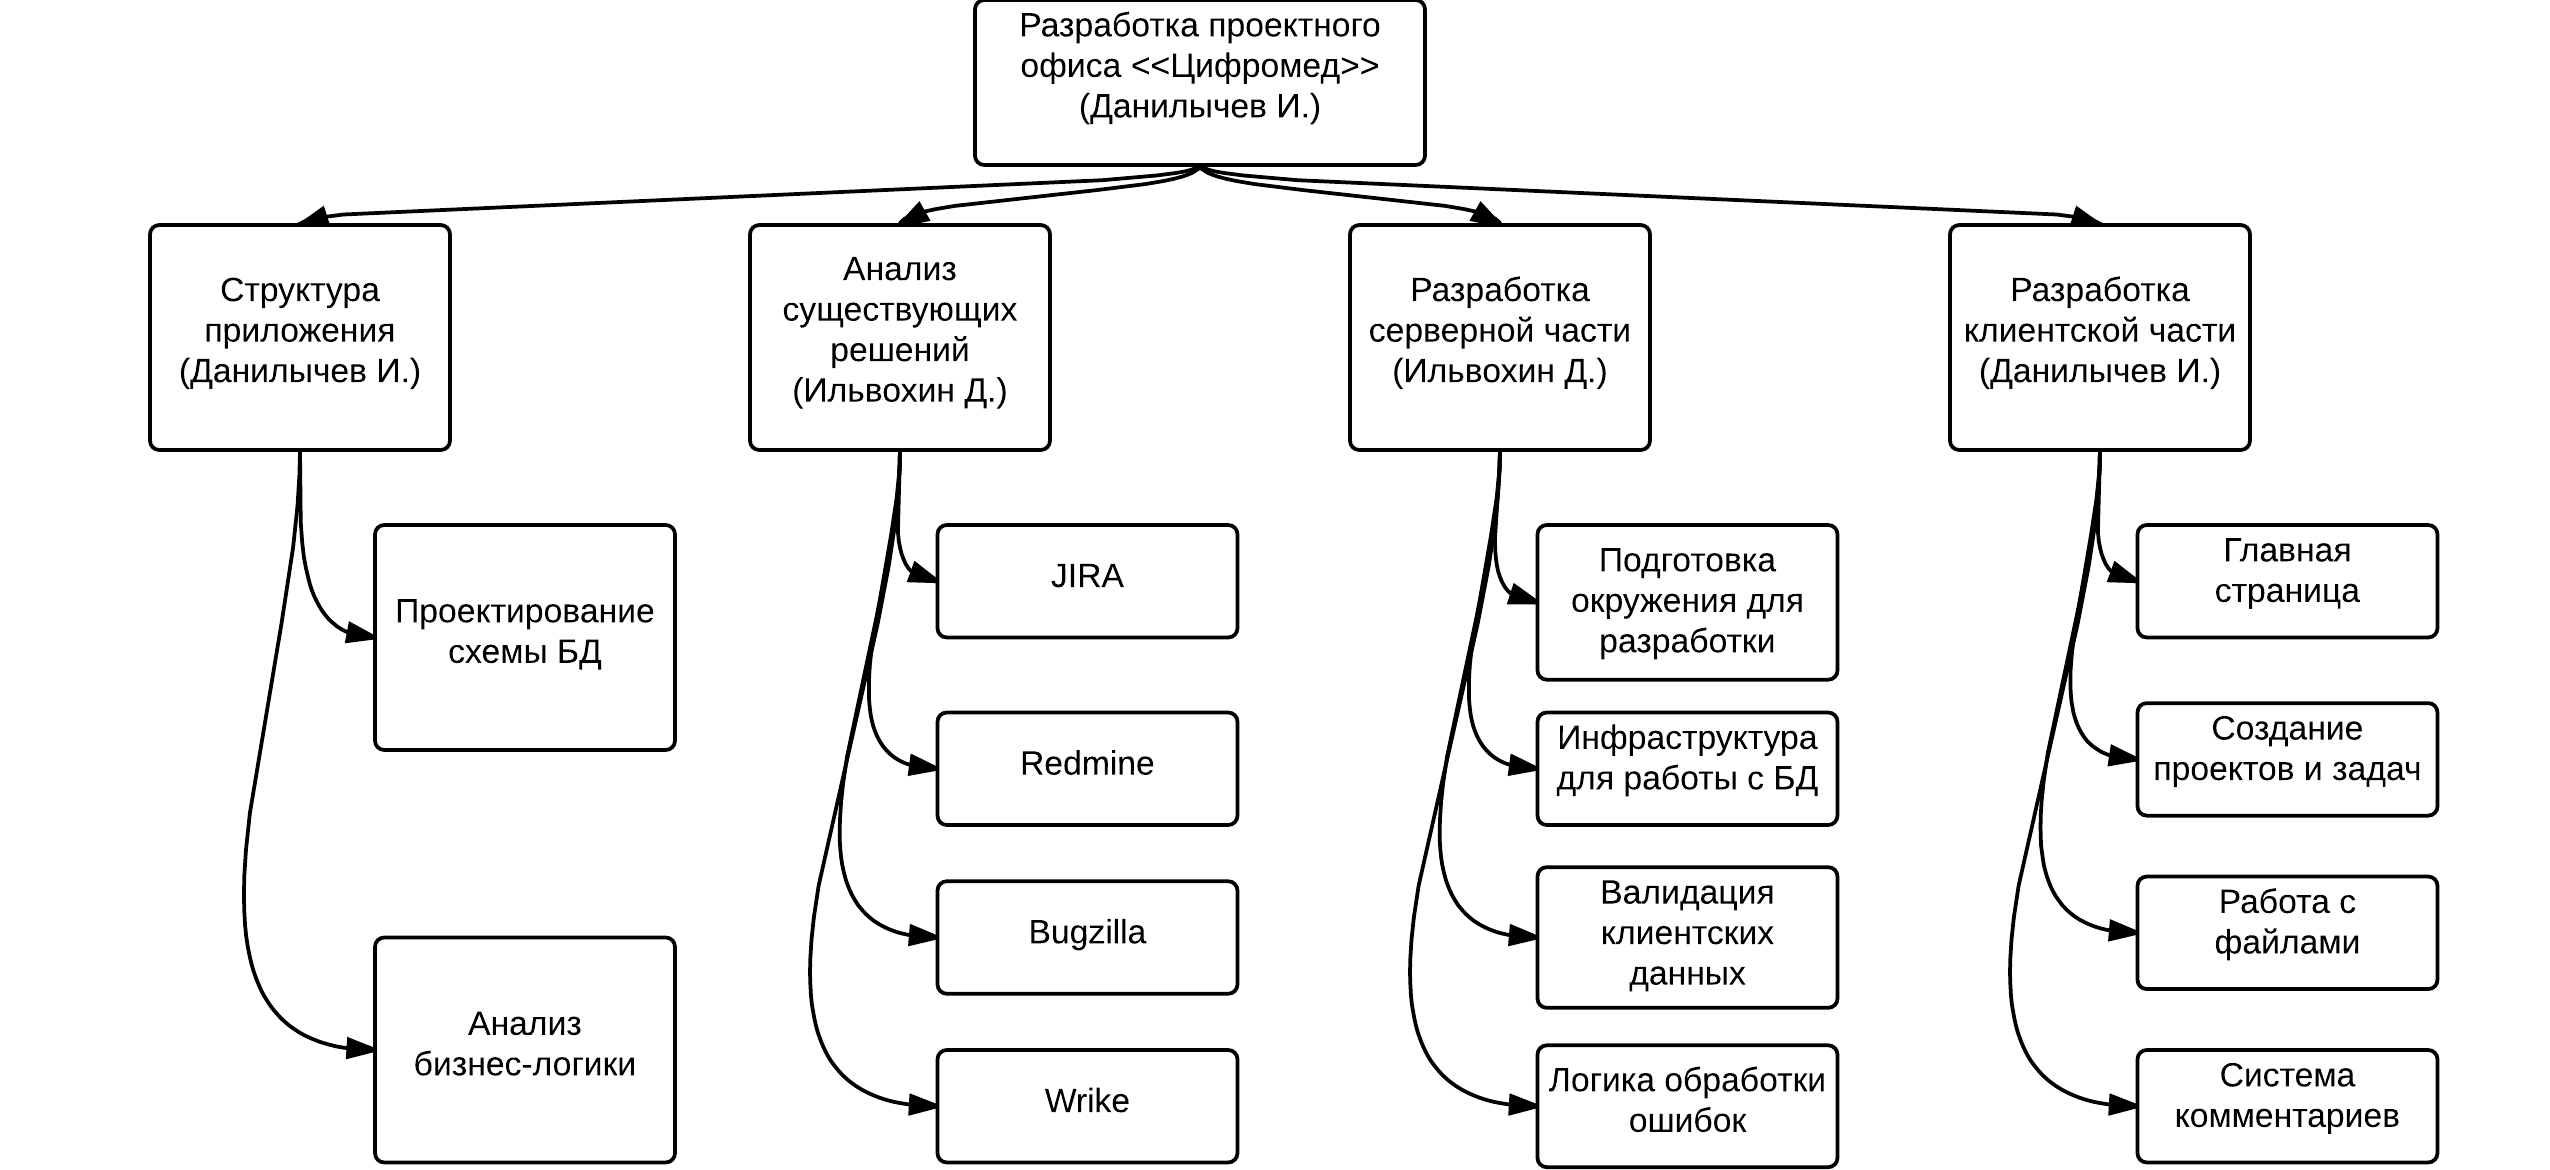
\includegraphics[scale=0.25]{../shared_images/wbs.png}
   \caption{Структура декомпозиции работ}
    \label{fig:start}
\end{figure}
\newpage


\subsection{Бизнес-модель проекта}

\begin{figure}[!htb]
  \centering
    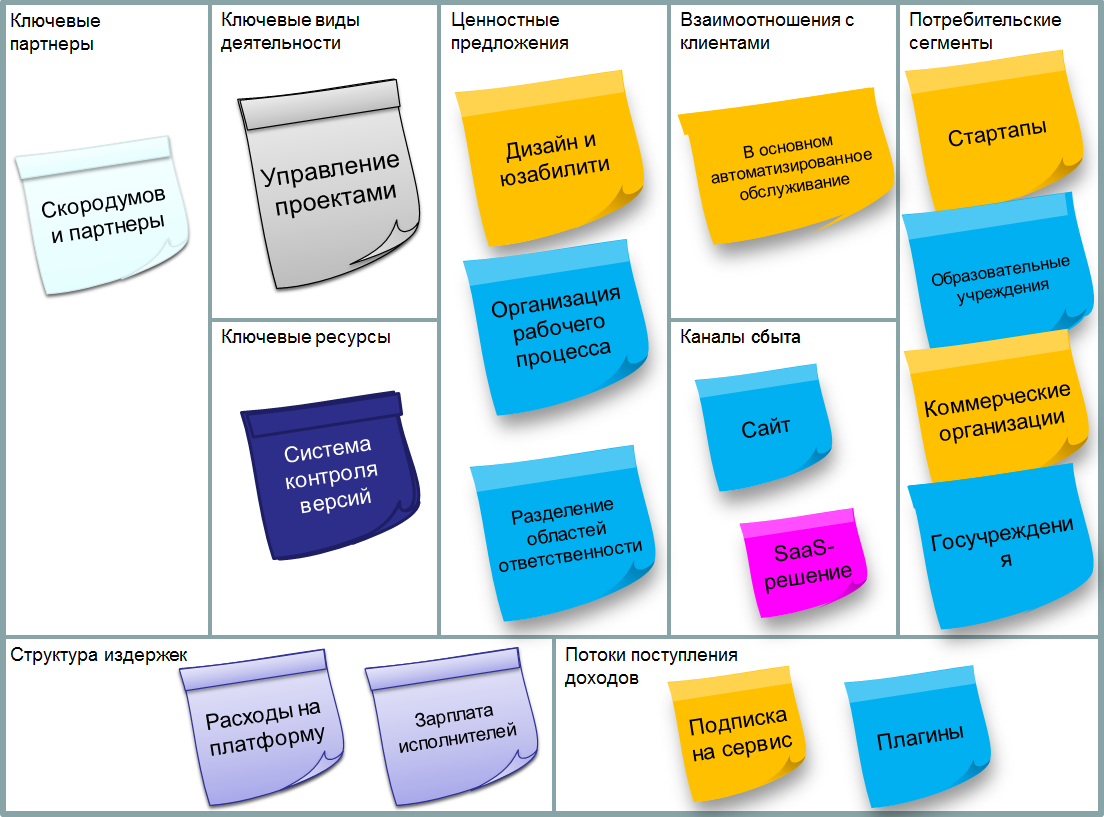
\includegraphics[scale=0.6]{../shared_images/business-model.png}
   \caption{Бизнес-модель проекта}
    \label{fig:start}
\end{figure}
  
Как видно из вышеприведённой модели, ключевым ресурсом проекта является децентрализованная система контроля версий. % Дописать про гит/гитхаб

В потребительские сегменты попали коммерческие, государственные и образовательные организации, а также стартапы. Потребители (клиенты) – сердце любой бизнес-модели. Без (выгодных) клиентов не может существовать ни одна компания. Чтобы лучше удовлетворять нужды клиентов, желательно разбить их на группы по потребностям, особенностям поведения или иным признакам. Так, для образовательных организаций стоит делать упор на низкую себестоимость данного решения, его простоту в освоении, доступность и пр.

Взаимоотношения с клиентами, благодаря самобалансируемости и самоподдерживаемости проекта, сводятся к минимуму; что же касается сервиса поддержки клиентов, он относится к вопросам монетизации (поступление доходов).

Ценностные предложения сводятся к реализации функций, описанных в цели проекта: организации рабочего процесса и взаимодействия проектных команд и членов проектов, разделения сфер ответственности и т.д., а также простому, минималистичному дизайну, который в данном случае, учитывая порой переусложнённые интерфейсы конкурентов, является скорей положительным фактором.

Создание и воплощение ценностных предложений, поддержание взаимоотношений с потребителями, получение прибыли – все эти процессы связаны с какими-либо издержками. Расходы достаточно легко подсчитать при уже определённых ключевых ресурсах, видах деятельности. В данном случае издержки сводятся к оплате труда программистов, работавших над проектным офисом, и расходам на поддержание офиса в рабочем состоянии (оплата хостинга и т.п.)

Наконец, потоки поступления доходов в данной модели представлены двумя возможностями. Первая -- продажа подписки на сервис поддержки клиентов, который будет обеспечивать техническое функционирование офиса на клиентской стороне (аналогичный подход используется многими компаниями, поставляющими SaaS-услуги, напр., Redmine). Вторая -- разработка встраиваемых компонент, или плагинов, по техническому заданию заказчика, которому недостает в стандартной поставке решения некоторых возможностей.


  \subsection{IDEF0}
  % Описание, диаграмма
  
  \subsection{DFD}
  % Описание, диаграмма

\newpage


\section{Техническое задание}
% Краткая аннотация, а затем -- задание из репозитория (с небольшими переработками)

\newpage


\section{Структура приложения}
  \subsection{Схема базы данных}
  % Описание, <<как пришли>> и схема
  
  \subsection{Бизнес-логика}
  % Много из http://habrahabr.ru/post/65432/
  
\newpage


\section{Серверная часть} % исправить заголовок?

\newpage


\section{Клиентская часть} % исправить заголовок?

\newpage


\section{Выводы}
% Ещё немного про то, что мы, безусловно, не конкуренты кому-либо, но наш проект можно использовать и вообще!

\newpage


\section{Паспорт проекта}
% Сырые PDF, экспортированные из MS Word; я не хочу перевёрстывать их в TeX

\end{document}